\documentclass[11pt]{article}

\usepackage[margin=1in]{geometry}
\usepackage{graphicx}
\usepackage[colorlinks=true]{hyperref}
\usepackage{siunitx}
\usepackage{listings}

% Set the listings programming language
\lstset{language=Matlab}

\begin{document}

MATH 373--01 (or --02, or --03)

Brent Deschamp

Homework \#1

January 31, 2018

\medskip\hrule\medskip

\section{Problem Statement}

Solve Kepler's equation, $E - e\sin{(E}) = M,$ when $e=0.048$ and $M = \pi/4$ using the methods of Bisection and False Position.

\section{Solution}

In order to determine an appropriate interval in which to search for a root, Kepler's equation was plotted for a range of $E$-values.  The results can be seen in Figure \ref{fig:kepler}.

\begin{figure}[h]
\begin{center}
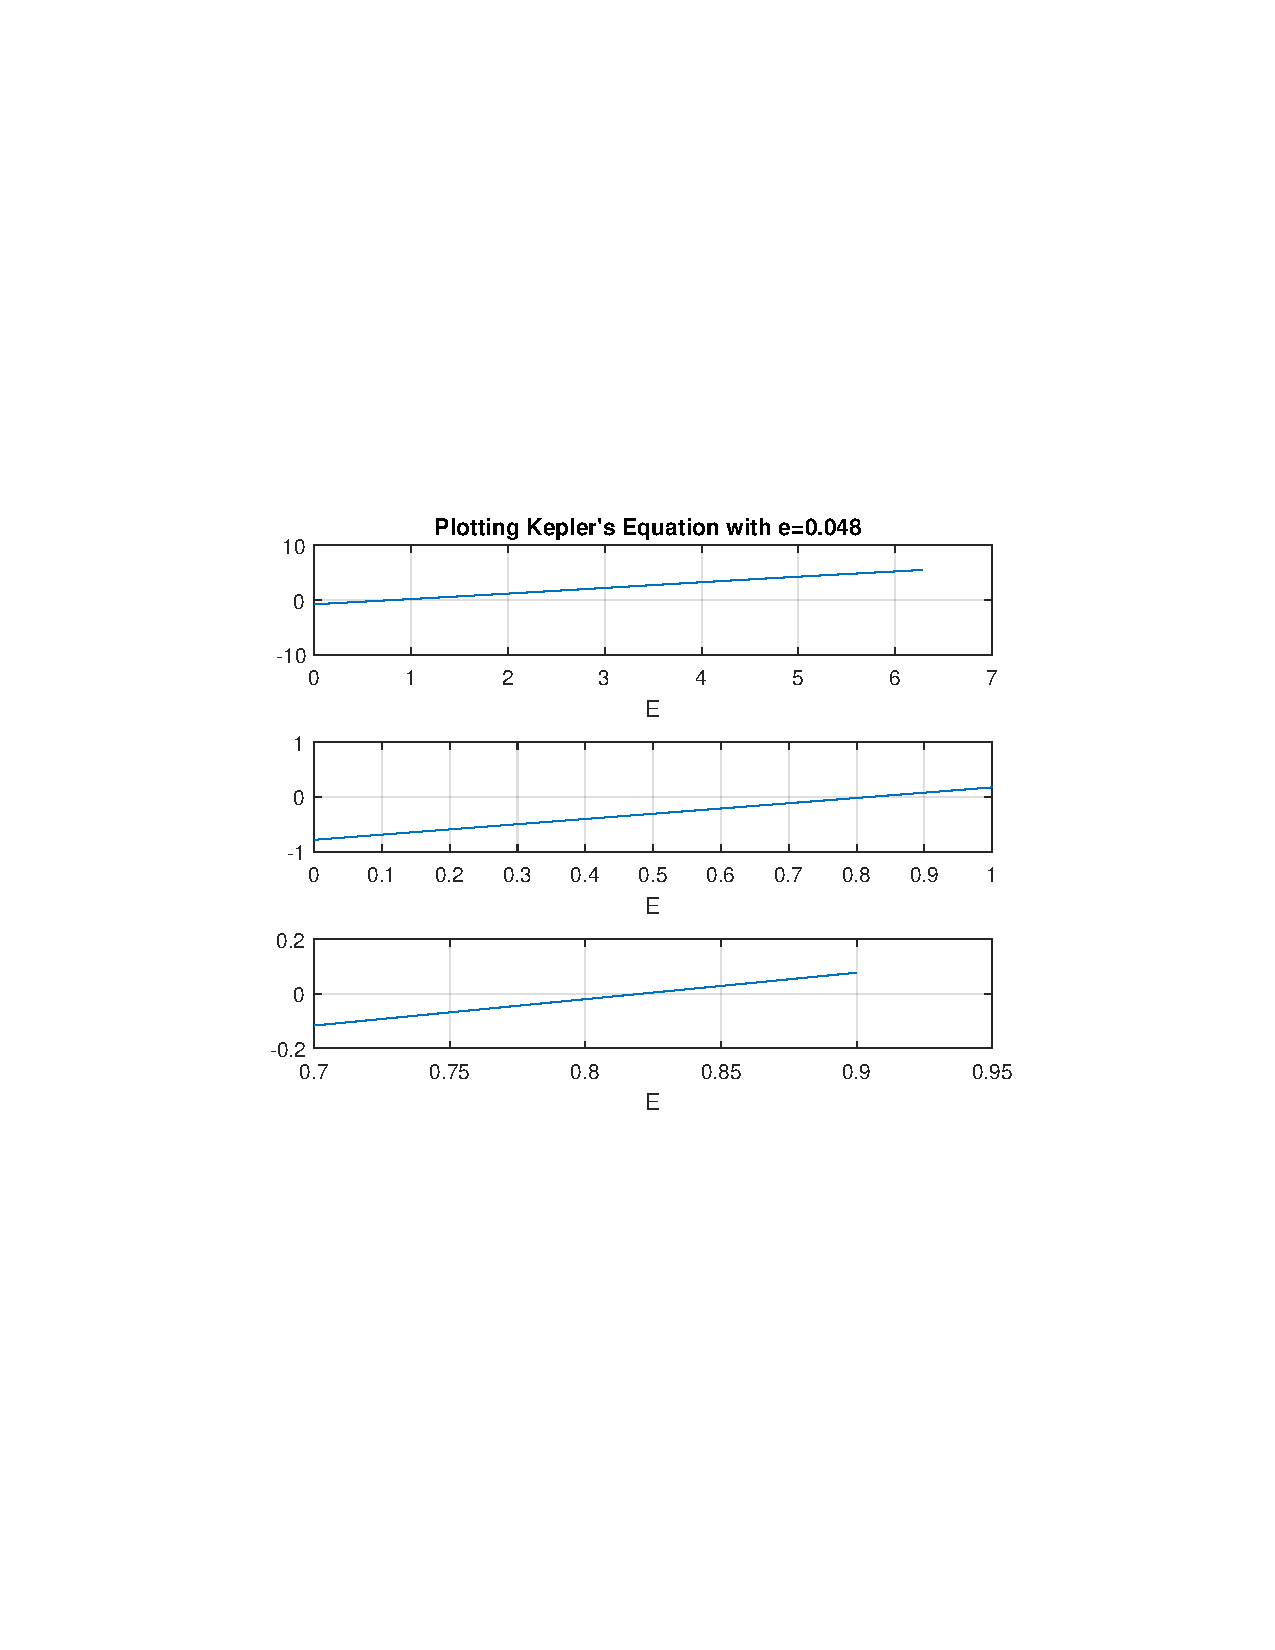
\includegraphics[trim={1.5in 3.55in 1.5in 3.25in},clip]{kepler_plot}
\caption{Plot of Kepler's equation.}\label{fig:kepler}
\end{center}
\end{figure}

An appropriate interval seems to be $[0.7,0.9]$, and the results of Bisection and False Position can be seen in Table \ref{table:kepler}.  Based on the methods, $E = 0.8205$ radians.  This value is reliable because the function value at the root is very small for both methods.  Also, the relative approximate error is small, and the methods terminated before reaching the maximum number of iterations, which is a good indication that the roots are accurate.

\renewcommand{\arraystretch}{1.2}

\begin{table}[h]
\begin{center}
\caption{Results from Bisection and False Position.}\label{table:kepler}
\smallskip
\begin{tabular}{l|cccc}
Method & \texttt{x\_root} & \texttt{func\_val} & $\varepsilon_a$ & Iterations\\\hline
Bisection & 0.8205 & \num{2.3856e-07} & \num{9.2984e-05} & 18\\
False Position & 0.8205 & \num{-3.6131e-10} & \num{3.0810e-05} & 3\\
\end{tabular}
\end{center}
\end{table}

\section{Command-line Usage}

Two programs were written to solve this problem, and the command-line usage is below.

\begin{verbatim}
>> Kepler_plot()

>> data = Kepler_problem()
\end{verbatim}

\section{Code}

The code for plotting Kepler's equation can be found in Listing \ref{code:plot}.  A program was written to solve this problem, called \texttt{Kepler\_problem}, and the code can be found in Listing \ref{code:problem}.  Note that \texttt{Kepler\_problem} calls the programs \texttt{bisection} and \texttt{false\_position}, but they are not included in this document.

\begin{lstlisting}[caption={MATLAB code for plotting Kepler's equation.}, label={code:plot}, frame=tb]
function Kepler_plot()
%%%%%%%%%%%%%%%%%%%%%%%%%%%%%%%%%%%%%
% Brent Deschamp
% August 23, 2016
% Plot Kepler's Equation: E-e*sin(E) = M

% No inputs

% No outputs.  Plots are automatically generated
%%%%%%%%%%%%%%%%%%%%%%%%%%%%%%%%%%%%%%%%

% Constants
e = 0.048;  % eccentricity for Jupiter
M = pi/4;   % mean anomaly

%%%%%%%%%%%%%%%%%%%%%%%%%%%%%%%

%Create values for E
E_vals = linspace(0,2*pi);
E_vals_finer = linspace(0,1);
E_vals_finer_still = linspace(0.7,0.9);

% Define function
Kepler = E_vals - e*sin(E_vals) - M;
Kepler_finer = E_vals_finer - e*sin(E_vals_finer) - M;
Kepler_finer_still = E_vals_finer_still - ...
	e*sin(E_vals_finer_still) - M;

% Plot the various functions
subplot(3,1,1);
plot(E_vals,Kepler);
xlabel('E');
grid
title(['Plotting Kepler''s Equation with e=' num2str(e)]);

subplot(3,1,2)
plot(E_vals_finer,Kepler_finer);
xlabel('E');
grid

subplot(3,1,3)
plot(E_vals_finer_still,Kepler_finer_still);
xlabel('E');
grid
\end{lstlisting}

%%%%%%%%%%%%%%%%%%%%%%%%%%%%%%%%%%%%%

\lstinputlisting[caption={MATLAB code for solving Kepler's equation.}, label={code:problem}, frame=tb]{Kepler_problem.m}

\end{document}